\begin{block}{Introduction: 2-D Vortex Patch Pair}
  A canonical problem in 2-D vortex dynamics is a steady
  translating pair of oppositely rotating vortex patches.

  \begin{minipage}[t]{0.45\linewidth}
    \begin{itemize}
    \item This problem was investigated \textit{numerically} a while
      back~\cite{pierrehumbert}.
    \item \textit{Mathematical analysis} has been limited to small
      vortices~\cite{marchioro-pulvirenti}.
    \end{itemize}
    \textbf{Objectives:}
    \begin{itemize}
    \item Prove existence of solution for vortices of any size.
    \item Provide analytical expressions for approximate solution.
    \end{itemize}
  \end{minipage}
  \hfill
  \begin{minipage}[t]{0.55\linewidth}
    \begin{figure}[h]\label{fig:pair}
      \centering
      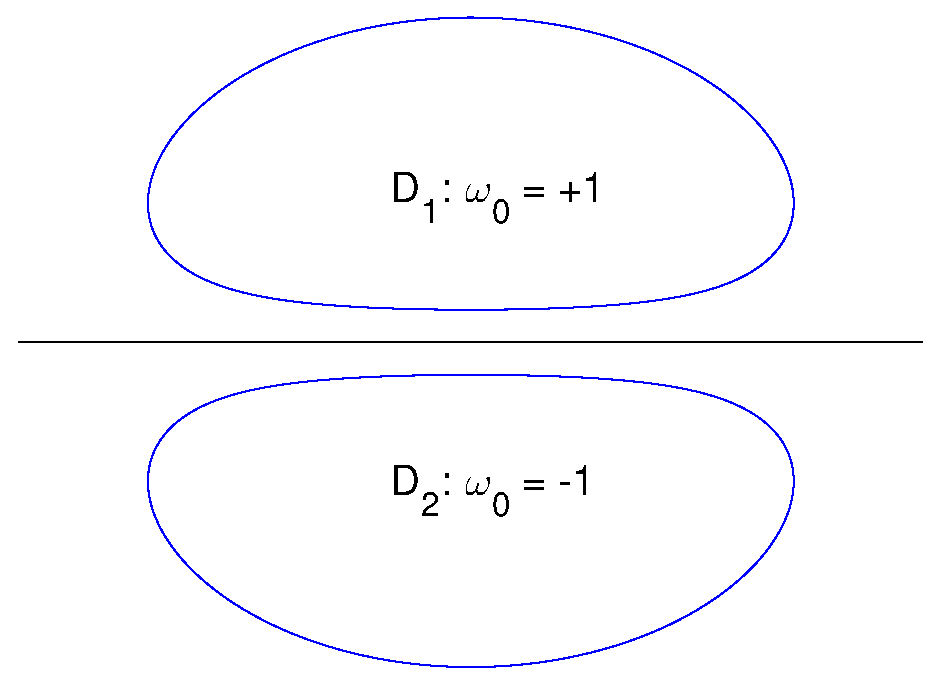
\includegraphics[width=1\linewidth]{pair}
      \caption{A stationary pair of vortex patches.}
    \end{figure}
  \end{minipage}
\end{block}

\begin{alertblock}{Statement of Problem}
  % \begin{alertblock}{Problem}
  For a given choice of length and vorticity $\om$, determine a simple
  differentiable closed curve $\partial D_1$, given by
  $z: [0, 2\pi] \rightarrow \mathbb{C}$, and a corresponding
  translation velocity $U$ so that
  \begin{equation}\label{eq:streamline}
    \im \left[\frac{\dd z}{\dd\nu} \frac{\dd w}{\dd z} \right] = 0
    \quad\text{on $\del D_1$,}
  \end{equation}
  where
  \begin{equation}\label{eq:dw/dz}
    \frac{\dd w}{\dd z}
    = -U + \frac{1}{4\pi} \int_{0}^{2\pi}
    \left(
      \frac{ \conj{z(\nu)-z(\nu')} }{ z(\nu)-z(\nu') }
      + \frac{ \conj{z(\nu)+z(\nu')} }{ z(\nu)+z(\nu') }
    \right)
    z'(\nu') \, \dd \nu'.
    % \frac{dz}{d\nu}(\nu') \,d\nu'.
  \end{equation}
  % \end{alertblock}
\end{alertblock}

% Example: Wingtip vortices
% %%%% Wingtip vortices
% \begin{figure}
%   \includegraphics[width=0.5\linewidth]{wingtip_vortices}
%   \caption{\footnotesize Credit: NASA Langley Research Center, Photo ID:~EL-1996-00130}
% \end{figure}
% %%%%%%%%%%%%%%%%%%%%%%%%%%%%%%%%%%%%%%%%%%%%%%%%%%%%%%%%%%%%%%%%%%%%

\begin{block}{Quasi-solution Method: General Procedures}
  Consider a nonlinear problem written abstractly as $\cN[w] =
  0$:
  \begin{itemize}
  \item Suppose one can find $w_{0}$ which satisfies initial and/or
    boundary conditions within a small error and the residual
    $\cR = \cN[w_{0}]$ is small.
  \item Then the error $E = w - w_0$ must satisfy
    \begin{equation}
      \label{eq:linear}
      \cL[E] = -\cR - \cN_{0}[E] \,,
    \end{equation}
    where $\cL = (\del\cN/\del w)|_{w=w_{0}}$ and
    $\cN_{0}[E] = \cN[w_{0}+E] - \cN[w_{0}] - \cL[E]$.
  \item If $\cL$ has a bounded inverse in some suitable space and
    $\cN_0$ is regular, then $E$ satisfies the weakly nonlinear
    equation
    \begin{equation}
      E = E_0
      - \cL^{-1} \cR - \cL^{-1} \cN_0 [E] \,,
    \end{equation}
    where $E_0$ is a solution to
    % the homogeneous linear problem
    $\cL E = 0$.
  \item The existence and uniqueness of solution to the nonlinear
    fixed point problem can be shown by the \textbf{contraction
      mapping principle}.
  \end{itemize}
\end{block}

\begin{block}{Challenges in Implementing QS Method}
  \begin{itemize}
  \item {\bf Nonlinearity}: the governing
    equation~\eqref{eq:streamline} is nonlinear in
    $z' (\nu)$.
    % since the complex velocity $dW/dz$ also involves $z'(\nu)$.
  \item {\bf Inversion of $\cL$}: need an equivalent formulation in
    which the Fr\'{e}chet derivative of the nonlinear operator at some
    approximate solution has a bounded inverse.
  \item {\bf Choice of solution space}: need to ensure that all
    nonlinear terms are controlled via Banach algebra property.
  \item {\bf Determination of scalar}: it is {\it a priori\/} unclear
    how to analytically determine velocity $U$ for given physical
    configuration.
    % separation of vortex centroids and choice of length and
    % vorticity scales.
  \end{itemize}
\end{block}
%%% Local Variables:
%%% mode: latex
%%% TeX-master: "main"
%%% End:
